%%%%%%%%%%
%
% Section: 3.2 Quadratic Equations, Functions, Zeros, and Models
% Author: John Hammond
%
%%%%%%%%%%

%%
%% Directions:
%% 1. Update the section's title and your name above
%% 2. Begin your edits beneath the %%%%%%%%% BEGIN HERE %%%%%%%%% line
%%
%% You can define terms like:
%% A \underline{quadratic equation} is an equation of the form \lgblank, where $a\ne 0$, and $a, b, c \in \mathbb{R}$. 
%%
%% Examples are of the form:
%% \begin{examples}[Directions here. Can be blank.]
%%   \ex This is an example \\[1in]     % it is up to you to specify appropriate spacing 
%% \end{examples}
%%
%%
\documentclass[11pt]{article}
\usepackage{workbook}
\begin{document}

%\tocsection{3.2:  Quadratic Equations, Functions, Zeros, and Models}


%%%%%%%%%%% BEGIN HERE %%%%%%%%%%%%%%%%%

\subsection*{Quadratic Equations and Functions}
A \underline{quadratic equation} is an equation of the form \lgblank, where $a\ne 0$, and $a, b, c \in \mathbb{R}$. \\[.15in]
A \underline{quadratic function} is a function of the form \lgblank, where $a\ne 0$, and $a, b, c \in \mathbb{R}$. \\[.15in]
Solving a quadratic equation is equivalent to finding the zeros of a quadratic function. \\[.15in]
\framebox{
\begin{tabular}{p{1in}|c|c|c}
\textbf{Graphs:} 
% 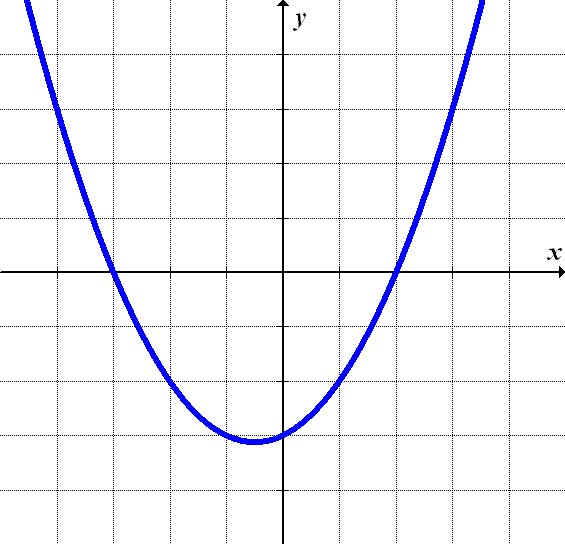
\includegraphics[width=1.75in]{teri/parabola2.png} &
% 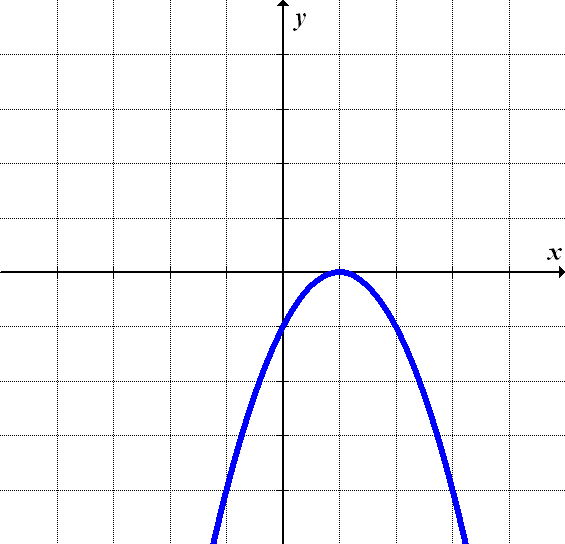
\includegraphics[width=1.75in]{teri/parabola1.png} &
% 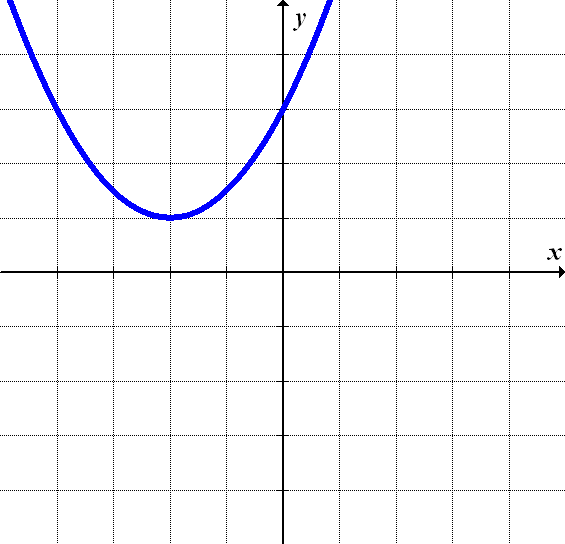
\includegraphics[width=1.75in]{teri/parabola0.png} \\ \hline 
& & & \\[-.1in]
\textbf{\# of $x$-int:} & & & \\ \hline
& & & \\[-.1in]
\textbf{\# of zeros:} & & & \\ \hline
& & & \\[-.1in]
\textbf{Discriminant:} & & & \\ \hline
 & & & \\[-.1in]
\textbf{Solutions:} & & & \\
\end{tabular}}

\vspace{.15in}

\begin{colbox}[Determine the nature of the solutions of the equation:]
\begin{tabular}{p{3.5in}p{3.5in}}
\ex $x^2-2x+4=0$ &
\ex $5t^2-7t=0$ \\[.5in]
\end{tabular}
\end{colbox}

\vspace{.15in}

\subsection*{Solving Quadratic Equations:}  We will employ three methods for solving quadratic equations:
\begin{enumerate}
\item FACTORING
\begin{colbox}[Solve by factoring:]
  \ex $5t^2-7t=0$ \\[.75in]
  \ex  $3x^2+x-2=0$ \\[.75in]
  \ex $x^2+4x=-4$\\[.75in]
\end{colbox}
\item COMPLETING THE SQUARE

Recall that $(x+A)^2 = x^2 + 2Ax + A^2$ is a perfect square trinomial.  Suppose we have an expression such as $x^2+18x$, and we want to add a constant so that it creates a perfect square:

$$x^2+18x+\xsblank = (\smblank)^2$$

\begin{colbox}[Solve by completing the square:]
  \ex $x^2-4x+2=0$ \\[1in]
  \ex $t^2+3t-7=0$ \\[1in]
  \ex $3x^2-6x-4=0$\\[1in]
  \ex $2z^2+3z-2=0$\\[1in]
\end{colbox}
\item THE QUADRATIC FORMULA (developed by completing the square on $ax^2+bx+c=0$)\\[.25in]
$$x=\lgblank$$

\vspace{.15in}
\noindent \mygrey{
\begin{tabular}{p{6.5in}}
\textbf{(EX)}  Solve using the quadratic formula:\\[.15in]
(a) $x^2-4x+2=0$ \\[.75in]
(b) $2z^2+3z-2=0$ \\[.75in]
\end{tabular}}

\end{enumerate}


\subsection*{Equations Reducible to Quadratic}
\noindent \mygrey{
\begin{tabular}{p{7in}}
\textbf{(EX)}  Solve:\\[.15in]
(a) $2x^4-9x^2=-4$ \\[1.5in]
(b) $x-8\sqrt{x}-9=0$ \\[1.5in]
(c) Find the zeros of the function:  $f(x) = x^{2/3} +3x^{1/3}-10$\\[1.5in]
(d) $2(t+2)^2-5(t+2)-12=0$\\[1.5in]
\end{tabular}}

\vspace{.15in}
\noindent \mygrey{
\begin{tabular}{p{7in}}
\textbf{(EX)}  The diagonal of a TV set is 30 inches long.  Its length is 12 inches less than twice the height.  Find the dimensions of the TV set.  \\[1.75in]
\end{tabular}}


\end{document}

